\documentclass{article}
\usepackage{graphicx}
\usepackage[left=1cm, right=1cm, top=2cm, bottom=2cm]{geometry}
\usepackage[russian]{babel}
\usepackage[T2A]{fontenc}
\usepackage[utf8]{inputenc}

\usepackage{listings}
\usepackage{xcolor}

\lstset{
	language=OCL,
	backgroundcolor=\color{gray!12}, % set backgroundcolor
	basicstyle=\ttfamily\small,%\footnotesize,% basic font setting
	commentstyle=\color{green!60!black},
	keywordstyle=\color{magenta},
	%stringstyle=\color{blue!50!red},
	%numbers=left,
	tabsize=4,
}

\title{Вариант 5.1а}
\author{Гусейнов Али}
\begin{document}
\maketitle
\tableofcontents
\clearpage
\section{Команда}
\section{Ресурсы}
	\subsection{Сетевой график}
	\subsection{Назначение ресурсов}
	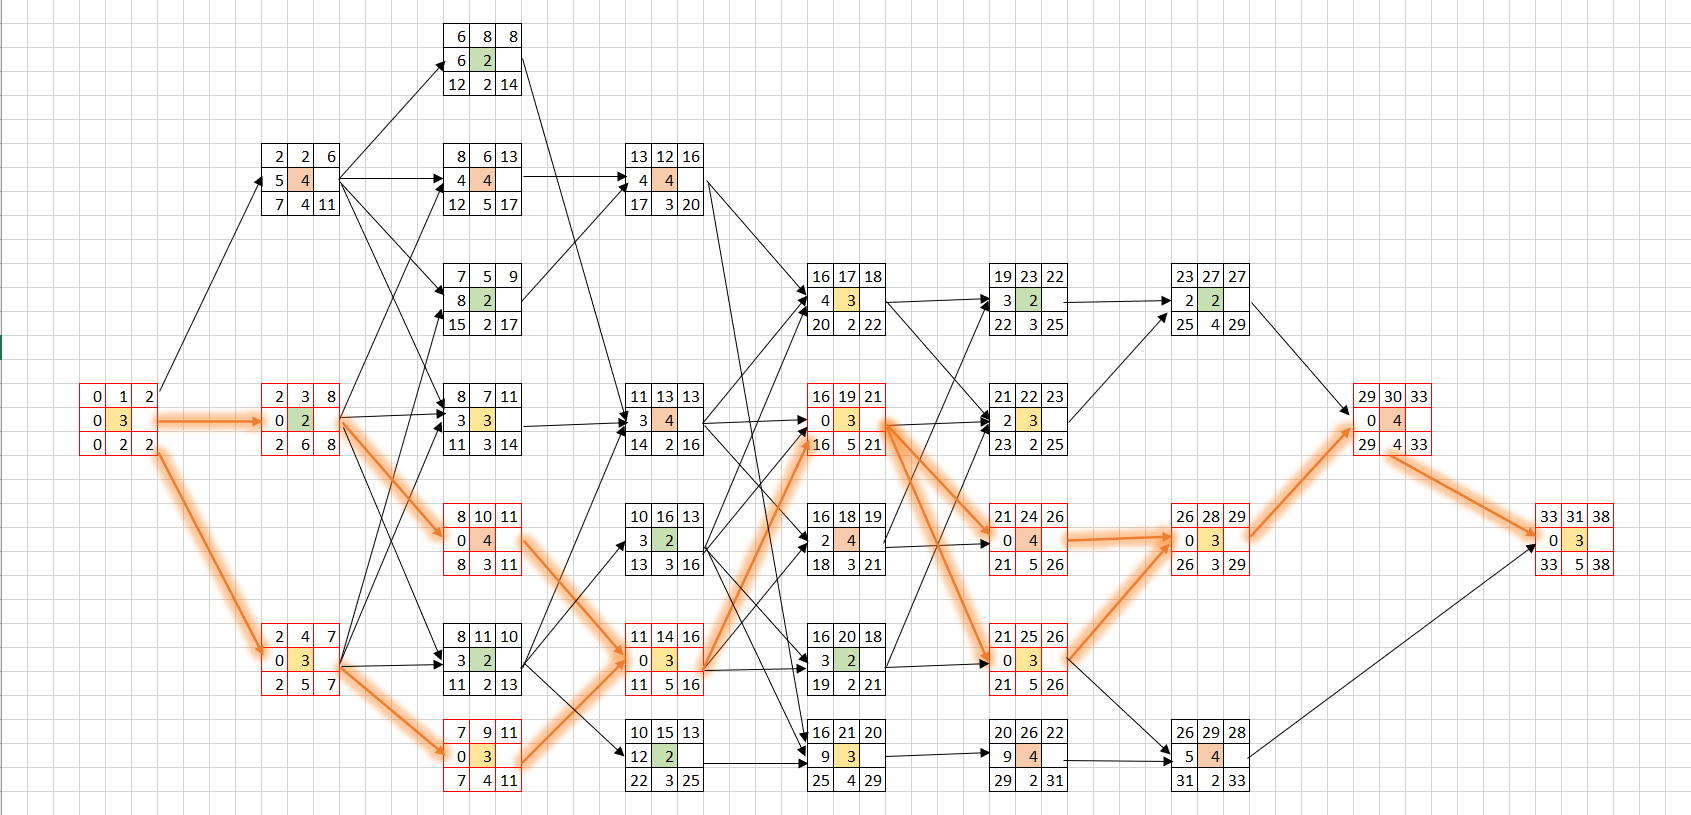
\includegraphics[width=\textwidth]{../img/init_network_graph.png}
\section{Первый способ}
	
\end{document}
